\documentclass[xcolor={dvipsnames,table},12pt]{beamer}

\usepackage[smartEllipses]{markdown}  % For markdown
\def\markdownOptionOutputDir{build}  % Needed, see https://github.com/Witiko/markdown/issues/6#issuecomment-328699108

\usepackage{array}
\usepackage{hyperref}
\usepackage{makecell}
\usepackage{comment}
\usepackage{xargs}
\usepackage{verbatim}
\usepackage{subfig}
\usepackage{booktabs}
\usepackage{changepage}
\usepackage{rotating, graphicx}
\usepackage{multirow}
\usepackage{pdflscape}
\usepackage{afterpage}
\usepackage[export]{adjustbox}
\usepackage[dvipsnames]{xcolor}
\usepackage[bottom]{footmisc}
\usepackage[colorinlistoftodos, prependcaption, textsize=tiny]{todonotes}

% References
\usepackage[backend=biber, style=numeric, sorting=none]{biblatex}
\usepackage{cleveref}

% Formatting
\setlength{\parindent}{0pt}
\setlength{\parskip}{1em}

% Encoding and languages
\usepackage[utf8]{inputenc}
\usepackage[english]{babel}
\usepackage[T1]{fontenc}        % För svenska bokstäver
%\usepackage[swedish]{babel}    %Svenska skrivregler och rubriker

% Graphics
\usepackage{epsfig}
%\usepackage[dvips]{graphics}

% For adding source captions to figures.
% From: https://tex.stackexchange.com/a/246285/36302
\newcommand{\source}[1]{\vspace{-0.3cm} \caption*{\footnotesize{Source: \textit{{#1}}}}}

\def\mytitleen{Classifying brain activity using electroencephalography and automated time tracking of computer use}
\def\mytitlesv{Klassificering av hjärnaktivitet med elektroencephalografi och automatiserad tidsspårning av datoranvändning}

\def\myauthor{Erik Bjäreholt}
\def\myorcid{0000-0003-1350-9677}
\def\myemail{erik@bjareho.lt}

\definecolor{LTHblue}{RGB}{0,0,128}
\definecolor{LTHbronze}{RGB}{156,97,20}

\newcommand\myshade{85}
\colorlet{mylinkcolor}{violet}
\colorlet{mycitecolor}{YellowOrange}
\colorlet{myurlcolor}{Aquamarine}

\hypersetup{%
  linkcolor=.,
  citecolor  = mycitecolor!\myshade!black,
  urlcolor = LTHblue,
  colorlinks = true,
}

% From: https://tex.stackexchange.com/a/173862/36302
\setbeamercolor*{structure}{bg=white,fg=LTHblue}

\setbeamercolor*{palette primary}{use=structure,fg=structure.fg,bg=structure.bg}
\setbeamercolor*{palette secondary}{use=structure,fg=white,bg=structure.fg!75}
\setbeamercolor*{palette tertiary}{use=structure,fg=white,bg=structure.fg!50!black}
\setbeamercolor*{palette quaternary}{fg=white,bg=black}

\setbeamercolor{section in toc}{fg=LTHblue,bg=white}
\setbeamercolor{alerted text}{use=structure,fg=structure.fg!50!black!80!black}

\setbeamercolor{titlelike}{fg=structure.fg!50!black}
\setbeamercolor{frametitle}{bg=white,fg=structure.fg}

\setbeamercolor*{titlelike}{parent=palette primary}

\bibliography{zotero}
\bibliography{misc}


% Formatting
\setlength{\parindent}{0pt}
\setlength{\parskip}{1em}

%Information to be included in the title page:
\title{\mytitleen}
\subtitle{\ \\ Master's thesis presentation}
\author{\myauthor}
\institute{Department of Computer Science\\Faculty of Engineering\\Lund University}
\date{October 28, 2021}

% Set font size for captions
%\usepackage{caption}
%\captionsetup{format=plain, font=scriptsize,labelfont=scriptsize}
\setbeamerfont{caption}{size=\scriptsize}

\newif\ifplacelogo{}  % create a new conditional
\placelogotrue{}      % set it to true
\logo{\ifplacelogo
\includegraphics[height=1.5cm]{LUlogoRGB.png}\fi}

\begin{document}

\frame{\titlepage}

\begin{frame}
    \begin{center}
        Abstract
    \end{center}
    {
        \scriptsizeWe investigate the ability of EEG to distinguish between different activities users engage in on their devices, building on previous research which showed a considerable difference in brain activity between code- and prose-comprehension, as well as differences during the synthesis. We explore multiple classification approaches, including using bandpass features, Riemannian geometry, and deep learning.

We also use the automated time tracker ActivityWatch to track what device activities the user is engaging in. This lets us label EEG data with naturalistic device activity, which we then use to train classifiers of device activity.

Code and a sample dataset is available at \href{https://github.com/ErikBjare/thesis}{github.com/ErikBjare/thesis}.

    }
\end{frame}

% What lead up to the thesis
\begin{frame}{Preface}
\framesubtitle{How it all began}

\begin{itemize}
    \item<1-> Pre-2013 --- Learning programming \& machine learning  % and Quantified Self
    \item<2-> 2013 --- Starting university
    \item<3-> 2015 --- ActivityWatch
    \item<4-> 2017 --- Finding the thesis project
    \item<5-> 2018 --- First experience using EEG
    \item<6-> 2020 --- Starting the thesis work
\end{itemize}
\end{frame}

\begin{frame}{Outline}
    \begingroup
        \setlength{\parskip}{0em}
        \tableofcontents
    \endgroup
\end{frame}

\section{Introduction}
\begin{frame}{Introduction}
    Before we begin, we will present two technologies used:

    \begin{itemize}
        \item Functional brain imaging
        \item Automated time trackers
    \end{itemize}
\end{frame}

\subsection{Functional brain imaging}
\begin{frame}{Introduction}
    \framesubtitle{Functional brain imaging}

    Functional brain imaging is used to measure aspects of brain function.

    Examples:
    \begin{itemize}
        \item Electroencephalography (EEG)
        \item Magnetoencephalography (MEG)
        \item Hemoencephalography (HEG)
        \item Functional Magnetic Resonance Imaging (fMRI)
        \item Functional Near-Infrared Spectroscopy (fNIRS)
    \end{itemize}
\end{frame}

\begin{frame}{Introduction}
    \framesubtitle{Functional brain imaging}

    Developments in the last $\sim$10 years:

    \begin{itemize}
        \item Cost reduction
        \item Consumer availability
    \end{itemize}

    Rough timeline:

    \begin{itemize}
        \item 2013: OpenBCI kickstarter
        \item 2016: InteraXon releases the Muse
        \item 2021: Neurosity releases the Crown
    \end{itemize}
\end{frame}

\begin{frame}{Introduction}
    \framesubtitle{Functional brain imaging}

    Applications:

    \begin{itemize}
        \item Discerning code vs prose comprehension
            \begin{itemize}
                \item Using MRI, by Floyd et al.~\cite{floyd_decoding_2017}
                \item Using EEG \& various biosensors, by Fucci et al.~\cite{fucci_replication_2019}
            \end{itemize}
        \item Neurolinguistics research
        \item Biofeedback / meditation aid
        \item Quantified self (measuring mood, focus)
    \end{itemize}
\end{frame}

\subsection{Automated time trackers}
\begin{frame}{Introduction}
    \framesubtitle{Automated time trackers}

    We use an automated time tracker to track which device activity a user is engaging in.

    Applications:
    \begin{itemize}
        \item Commercial use
        \item Research use
    \end{itemize}

    Examples:
    \begin{itemize}
        \item RescueTime (commercial use)
        \item TimeAware (research use)
        \item Screen Time (Apple)
        \item Digital Wellness (Android)
    \end{itemize}
\end{frame}


\begin{frame}{Introduction}
    \framesubtitle{Automated time trackers}

    Issues with existing solutions:
    \begin{itemize}
        \item Data resolution
        \item Source availability / licensing
        \item Privacy concerns
    \end{itemize}
\end{frame}

\placelogofalse{}
\begin{frame}{Introduction}
    \framesubtitle{Automated time trackers}

    \begin{columns}
        \begin{column}{0.5\textwidth}
            \hspace{0.4em}
            \begingroup
                \scriptsize
                Our solution:
                \\
            \endgroup
            \vspace{0.2em}
            \hspace{0.4em}
            \begingroup
                \large
                ActivityWatch
            \endgroup
            \vspace{0.5em}

            \begin{itemize}
                \item{\emph{``The world's best free \& open-source automated time tracker''}}
                \item Started in 2015 by me
                \item My brother joined in 2016
                \item ${>}100{,}000$ downloads
                \item ${>}90$ contributors
                \item Available on Windows, macOS, Linux, and Android.
            \end{itemize}

            \vfill
        \end{column}
        \begin{column}{0.6\textwidth}
            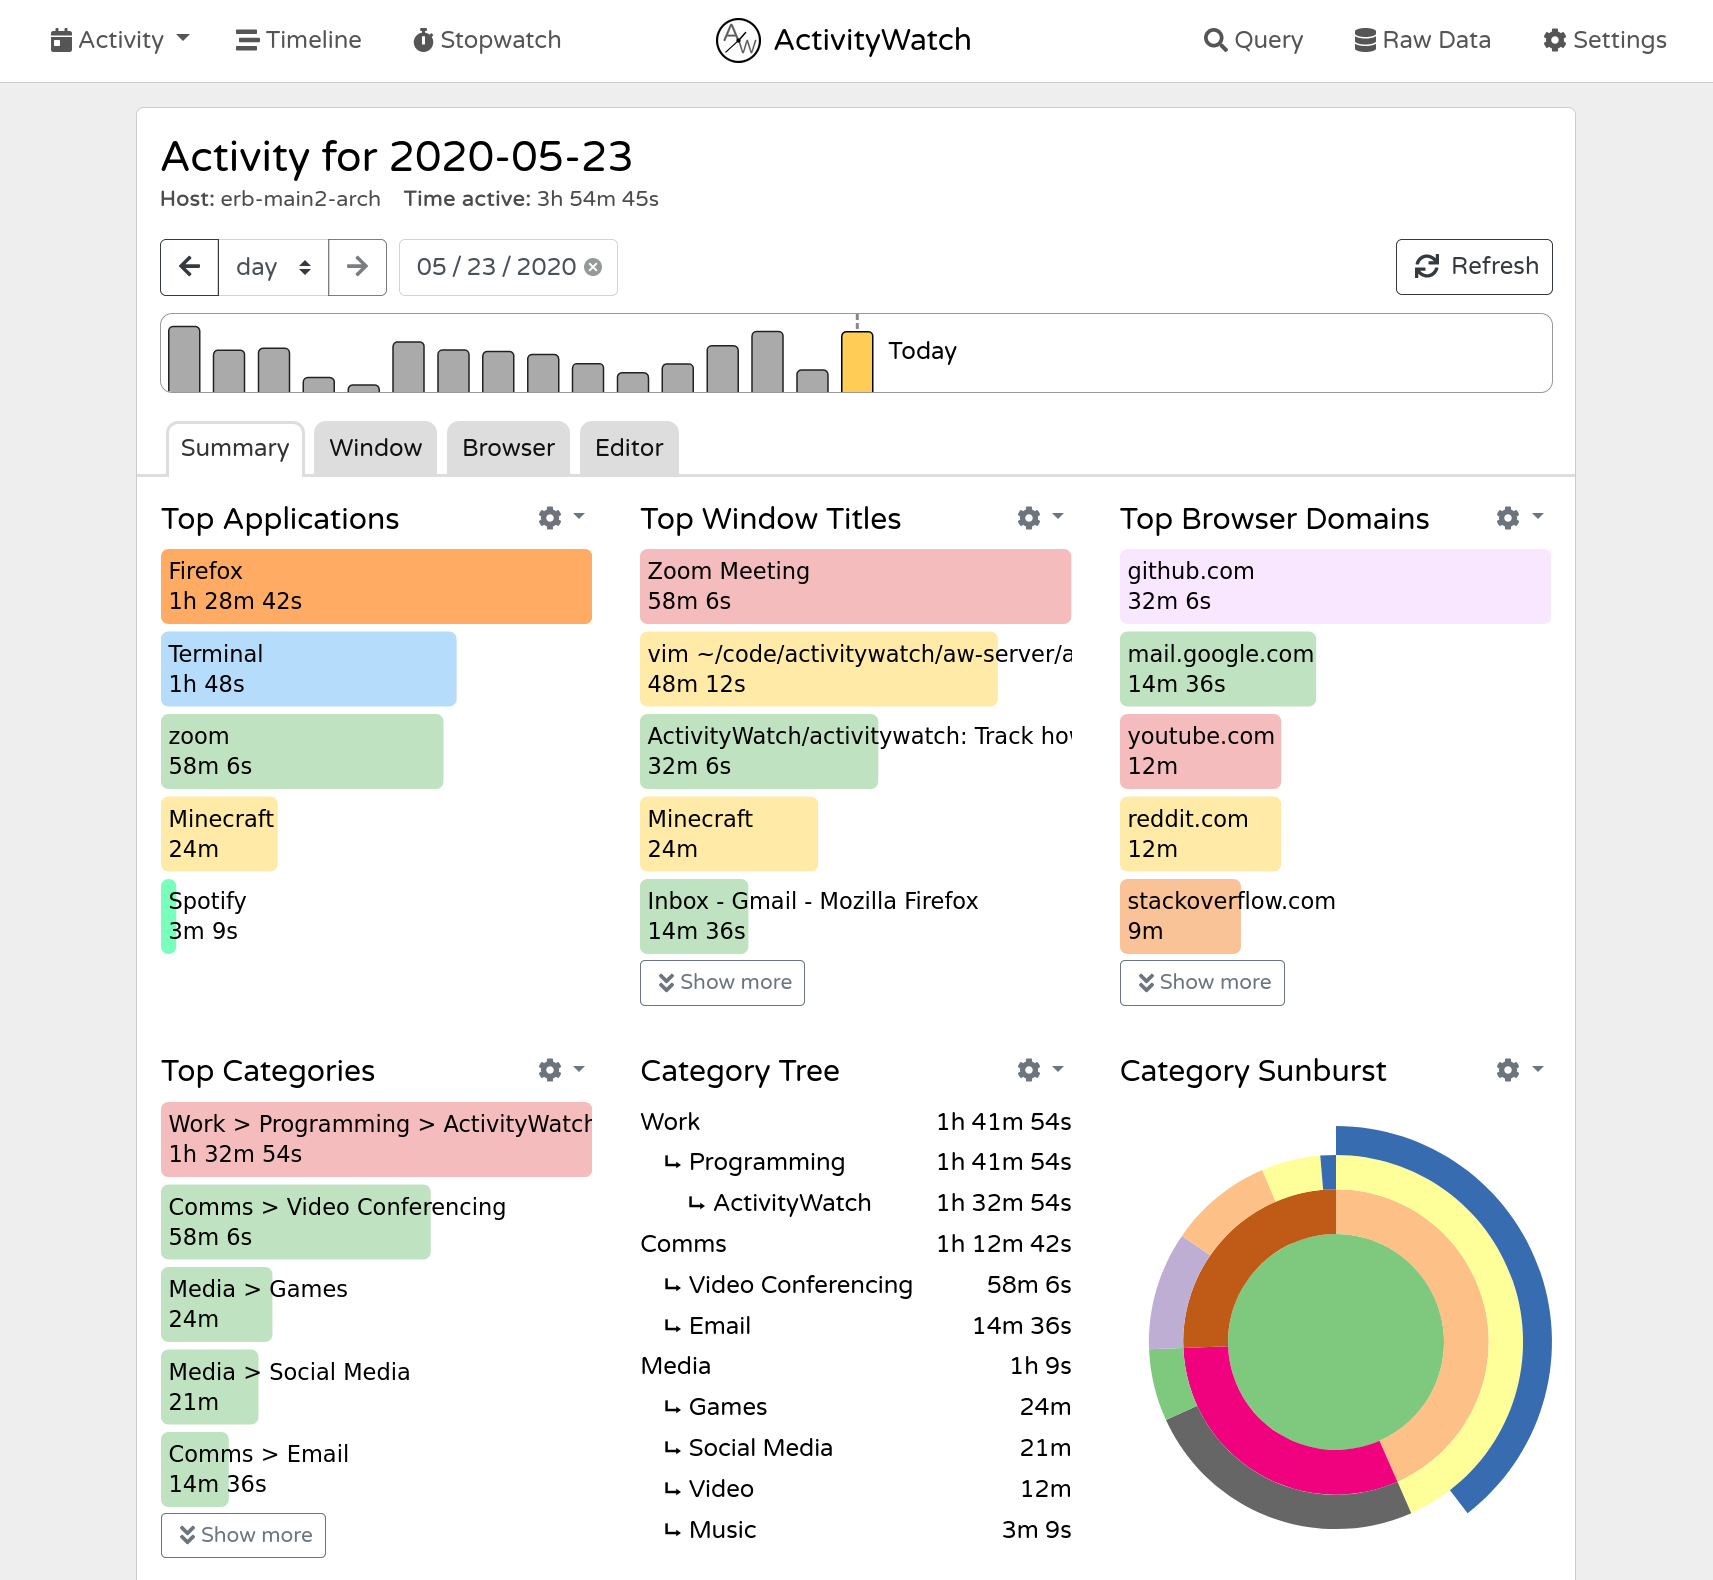
\includegraphics[width=\textwidth]{img/screenshot-aw-activity.png}
        \end{column}
    \end{columns}
\end{frame}
\placelogotrue{}

\section{Theory}
\begin{frame}{Theory}
    This thesis rests on theory within electroencephalography and machine learning.
\end{frame}

\subsection{Electroencephalography}
\begin{frame}{Theory}
    \framesubtitle{Electroencephalography}

    EEG is\ldots

    ERPs...

    The 10-20 system...

    Frequency bands...
\end{frame}

\placelogofalse{}
\begin{frame}{Theory}
    \framesubtitle{Electroencephalography}
    \vspace*{-5mm}

    \begin{figure}
        \hspace*{-10mm}
        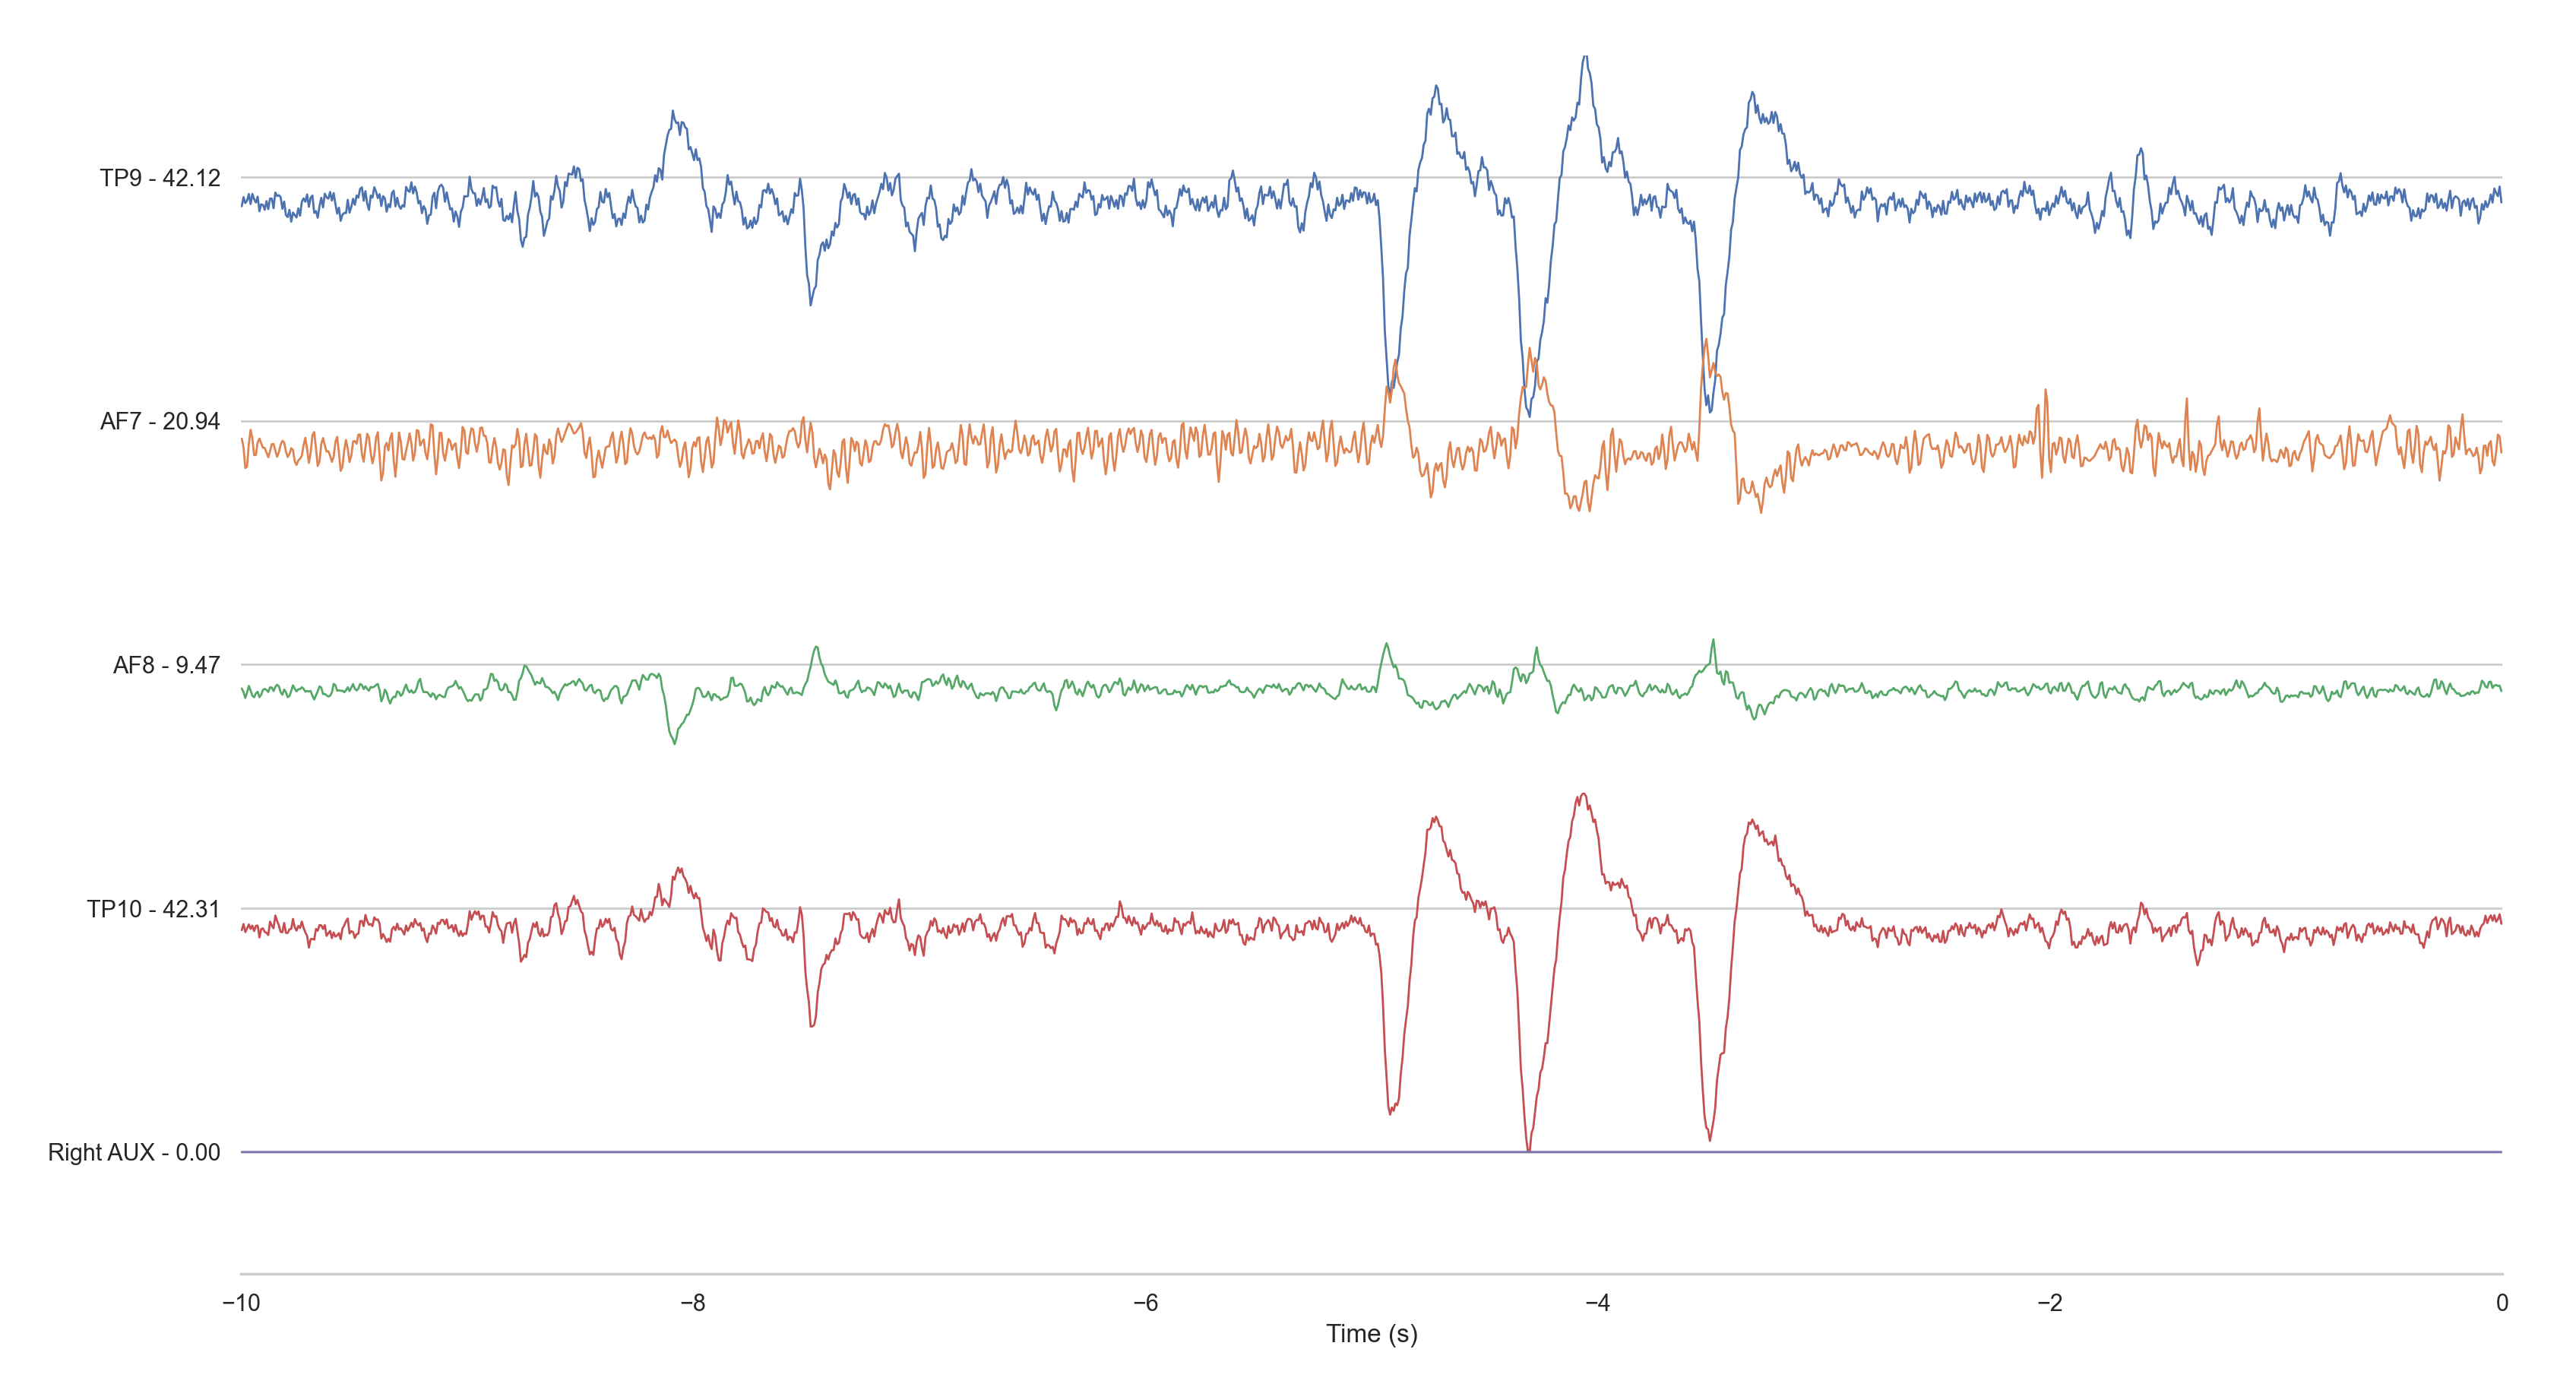
\includegraphics[width=\paperwidth]{img/muselsl-signal.png}
        \caption{Example of EEG data, viewed with muse-lsl. Three eye blinks clearly visible around $-4s$.}
    \end{figure}
\end{frame}
\placelogotrue{}

\subsection{Machine learning}
\begin{frame}{Theory}
    \framesubtitle{Machine learning}
\end{frame}

\begin{frame}{Theory}
    \framesubtitle{Machine learning $>$ Riemannian geometry}
    
    Riemannian methods in EEG utilizes the spatial information encoded in covariance matrices to estimate the similarity between two signals.
    \\
    \vspace{1em}
    In the simple \emph{Minimum Distance to Mean} (MDM) method, matrices for each class are averaged in Riemannian space. For a new signal's matrix, the distance to each class is calculated, and whichever class distance is smaller becomes the predicted class.
\end{frame}

\begin{frame}{Theory}
    \framesubtitle{Machine learning $>$ Riemannian geometry}
    
    \small The Riemannian distance metric $\delta_G$ for two symmetric positive definite matrices $A$ and $B$ (such as covariance matrices) is~\cite{grafarend_metric_2003}:

        \[ \delta_G(A, B) = \sqrt{\sum_{i=1}^N \log^2 \lambda_i (A, B) } \]
\end{frame}

\begin{frame}{Theory}
    \framesubtitle{Machine learning $>$ Riemannian geometry}
    {
        \scriptsize
        \begin{figure}[h]
    \centering
    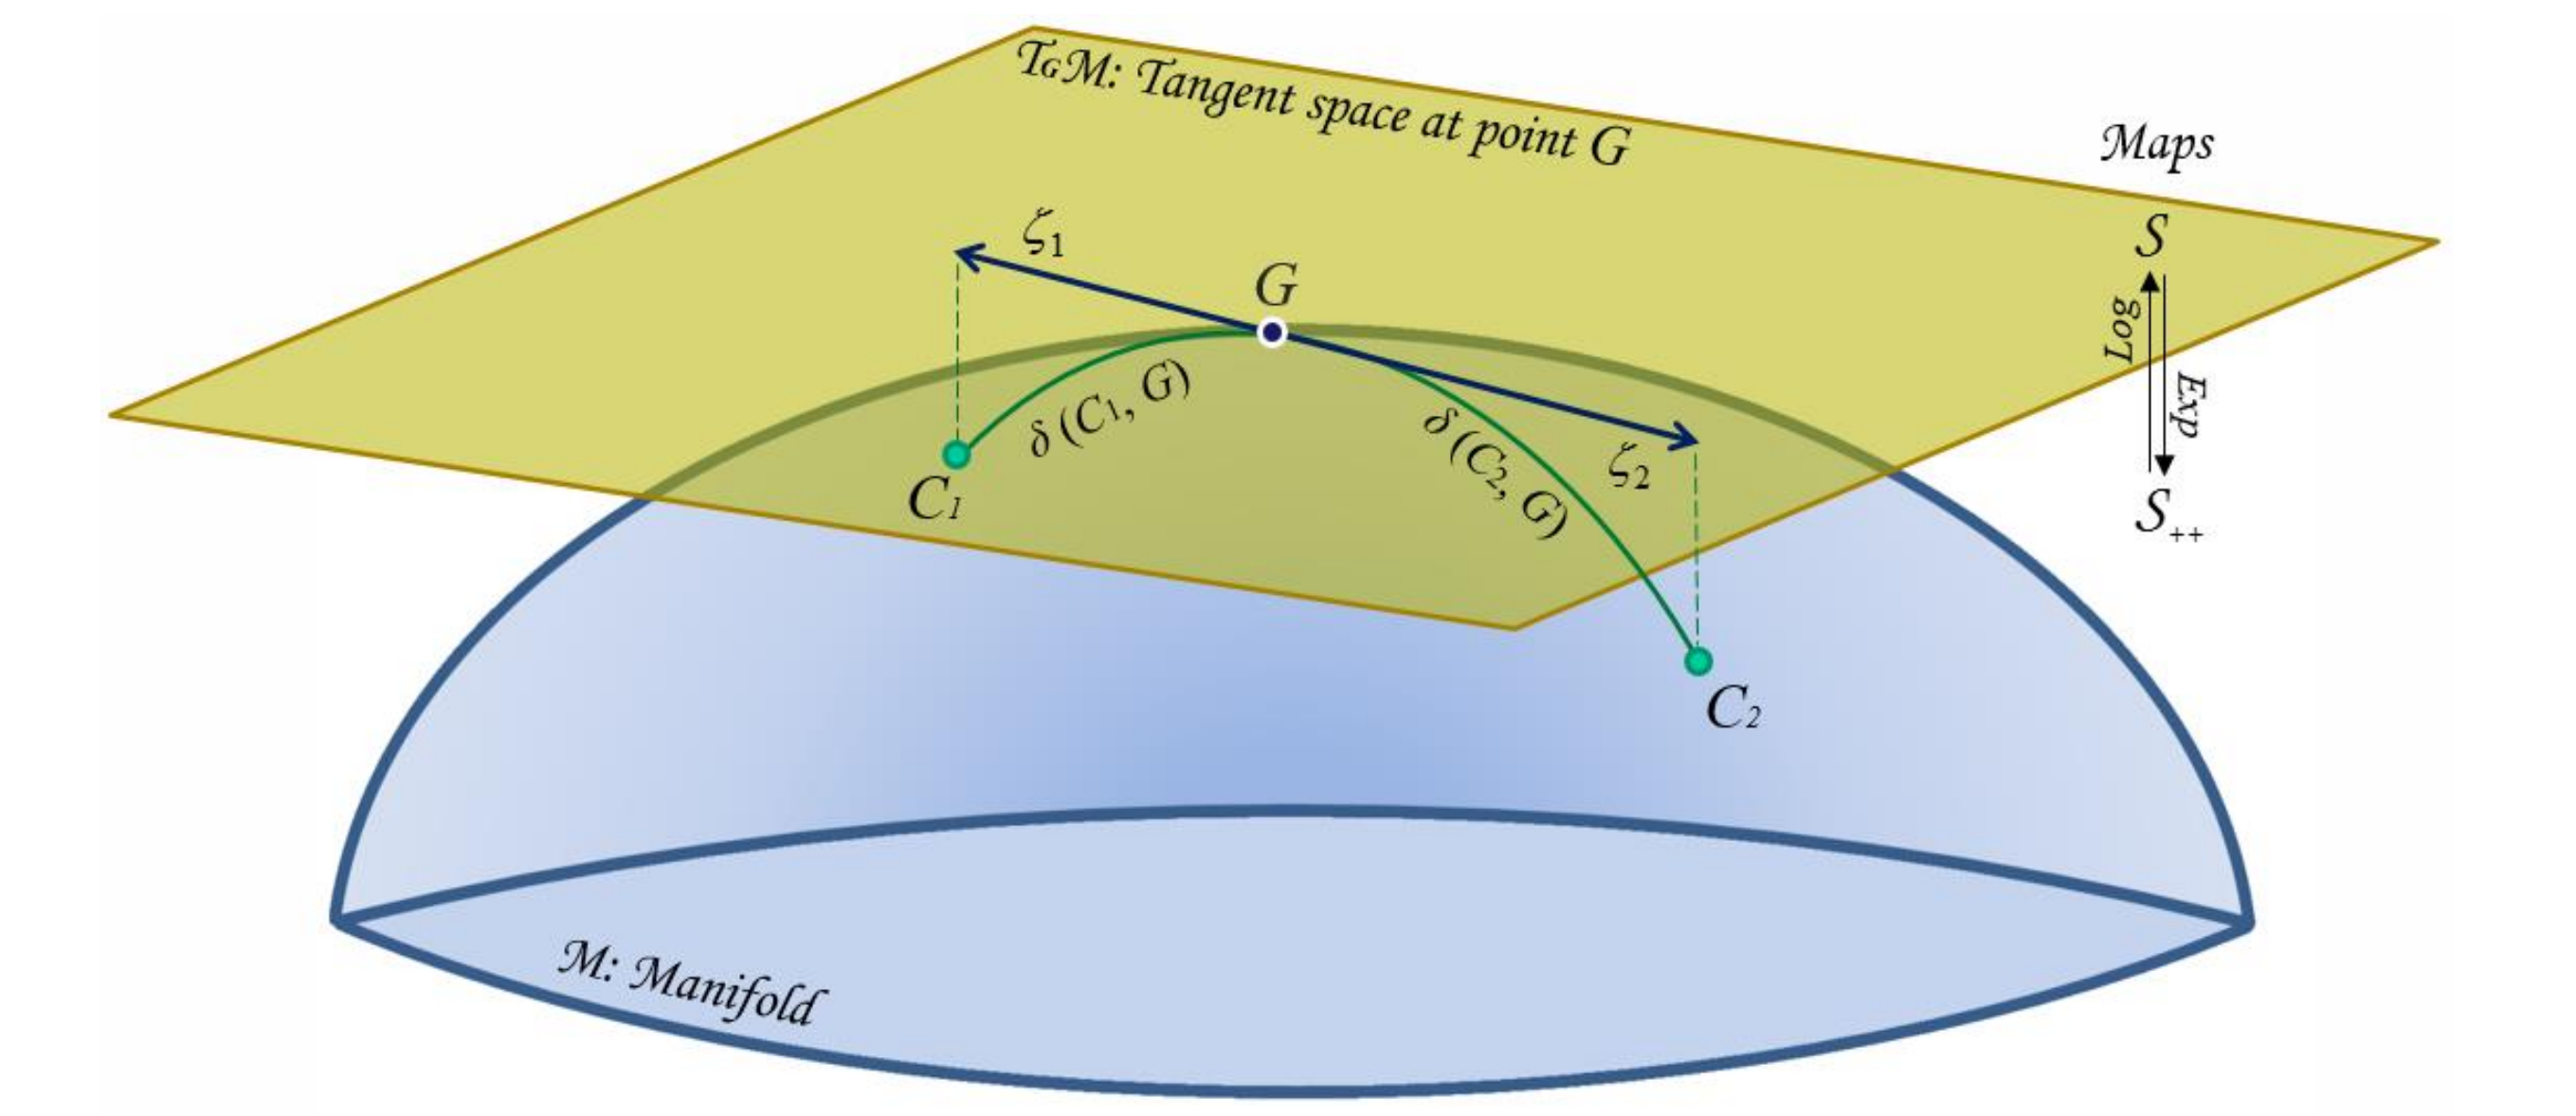
\includegraphics[width=0.6\textwidth]{img/riemannian-tangent-space.png}
    \caption{Schematic representation of the symmetric positive definite matrix manifold, the geometric mean $G$ of two points and the tangent space at $G$. The geometric mean of these points is the midpoint on the geodesic connecting $C_1$ and $C_2$, i.e.\ it minimizes the sum of the two squared distances. The map from the tangent space to the manifold is an exponential map. The inverse map is a logarithmic map.}\label{figure:tangent-space}
    \source{Congedo et al.~\cite{congedo_riemannian_2017}}
\end{figure}

    }
\end{frame}

\section{Method}
\begin{frame}{Method}
    \includegraphics[width=\textwidth]{img/method.png}
\end{frame}

\placelogofalse{}
\begin{frame}{Method}
    \framesubtitle{Comparison with previous studies}
    \vspace*{-10mm}
    \begin{adjustbox}{width=\textwidth,center,float=table}
        \rowcolors{4}{gray!25}{white}
\begin{table}
    \begin{center}
        \begin{tabular}{llll}
            \toprule
            \multirow{2}{*}{\textbf{Setting}} & \multicolumn{3}{c}{\textbf{Study}} \\
            \cmidrule(lr){2-4}
            & \makecell[c]{\textbf{This study}} & \makecell[c]{\textbf{Fucci et al.} (2019)} & \makecell[c]{\textbf{Floyd et al.} (2017)} \\
            \midrule
            Experiment site & Lund Univ. (Sweden) & Univ.\ of Bari (Italy) & Univ.\ of Virginia (USA)  \\
            \# Participants & 9 & 28 & 29 \\
            Participants experience & Grads & Undergrads & Grads \& Undergrads \\
            \# Tasks & Variable & 36 tasks & 27 tasks \\
            Task type & \makecell[l]{Code comprehension \\ Prose review} & \makecell[l]{Code comprehension \\ Prose comprehension} & \makecell[l]{Code comprehension \\ Code review \\ Prose review} \\
            Physiological signal & Neural & \Gape[0pt][2pt]{\makecell[l]{Neural \\ Skin \\ Heart}} & Neural \\
            Physiological measure & EEG & \makecell[l]{EEG \\ EDA \\ HR, HRV, BVP} & BOLD \\
            Device & Muse S & \Gape[0pt][2pt]{\makecell[l]{BrainLink Headset \\ Empatica wristband}} & fMRI \\
            Classifier & Riemannian geometry & 8 algorithms & Gaussian Process \\
            Classifier validation & LORO-CV & \Gape[0pt][2pt]{\makecell[l]{LORO-CV \\ Hold-out}} & LORO-CV \\
            Classifier metric & Balanced accuracy (BAC) & Balanced accuracy (BAC) & Balanced accuracy (BAC) \\
            \bottomrule
        \end{tabular}
        \caption{Comparison of this study's method with previous studies.}\label{table:compare-method}
    \end{center}
\end{table}
\rowcolors{2}{}{}

    \end{adjustbox}
\end{frame}
\placelogotrue{}

    \subsection{Devices}
\begin{frame}{Method}
    \framesubtitle{Devices}

    \begin{columns}
        \begin{column}{0.33\textwidth}
            \vspace{9mm}
            \centering
            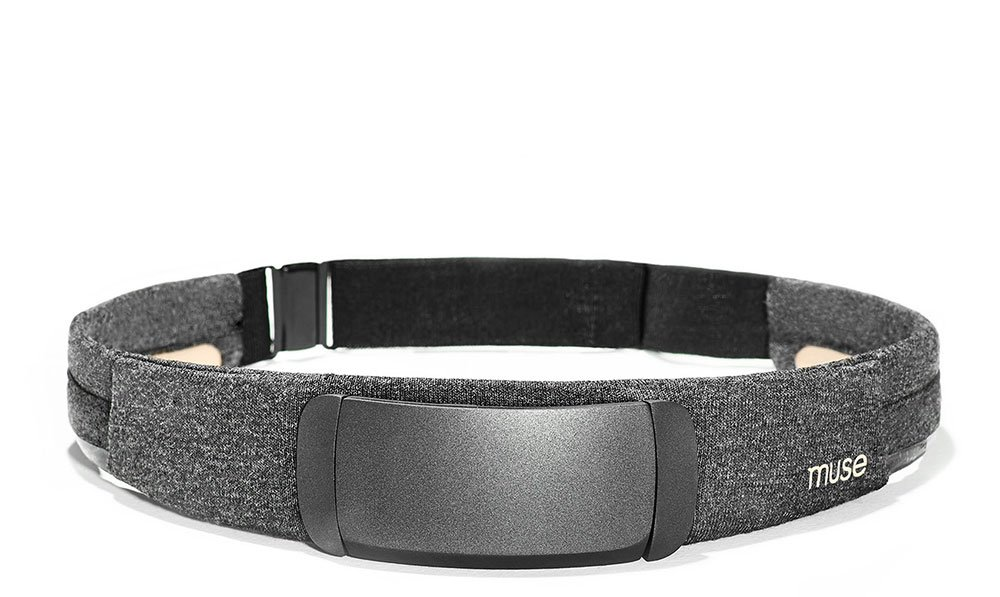
\includegraphics[trim=0 -50 0 200,clip,width=\textwidth]{./img/Muse-S.jpg}
            \\ Muse S
        \end{column}

        \begin{column}{0.33\textwidth}
            \vspace{4mm}
            \centering
            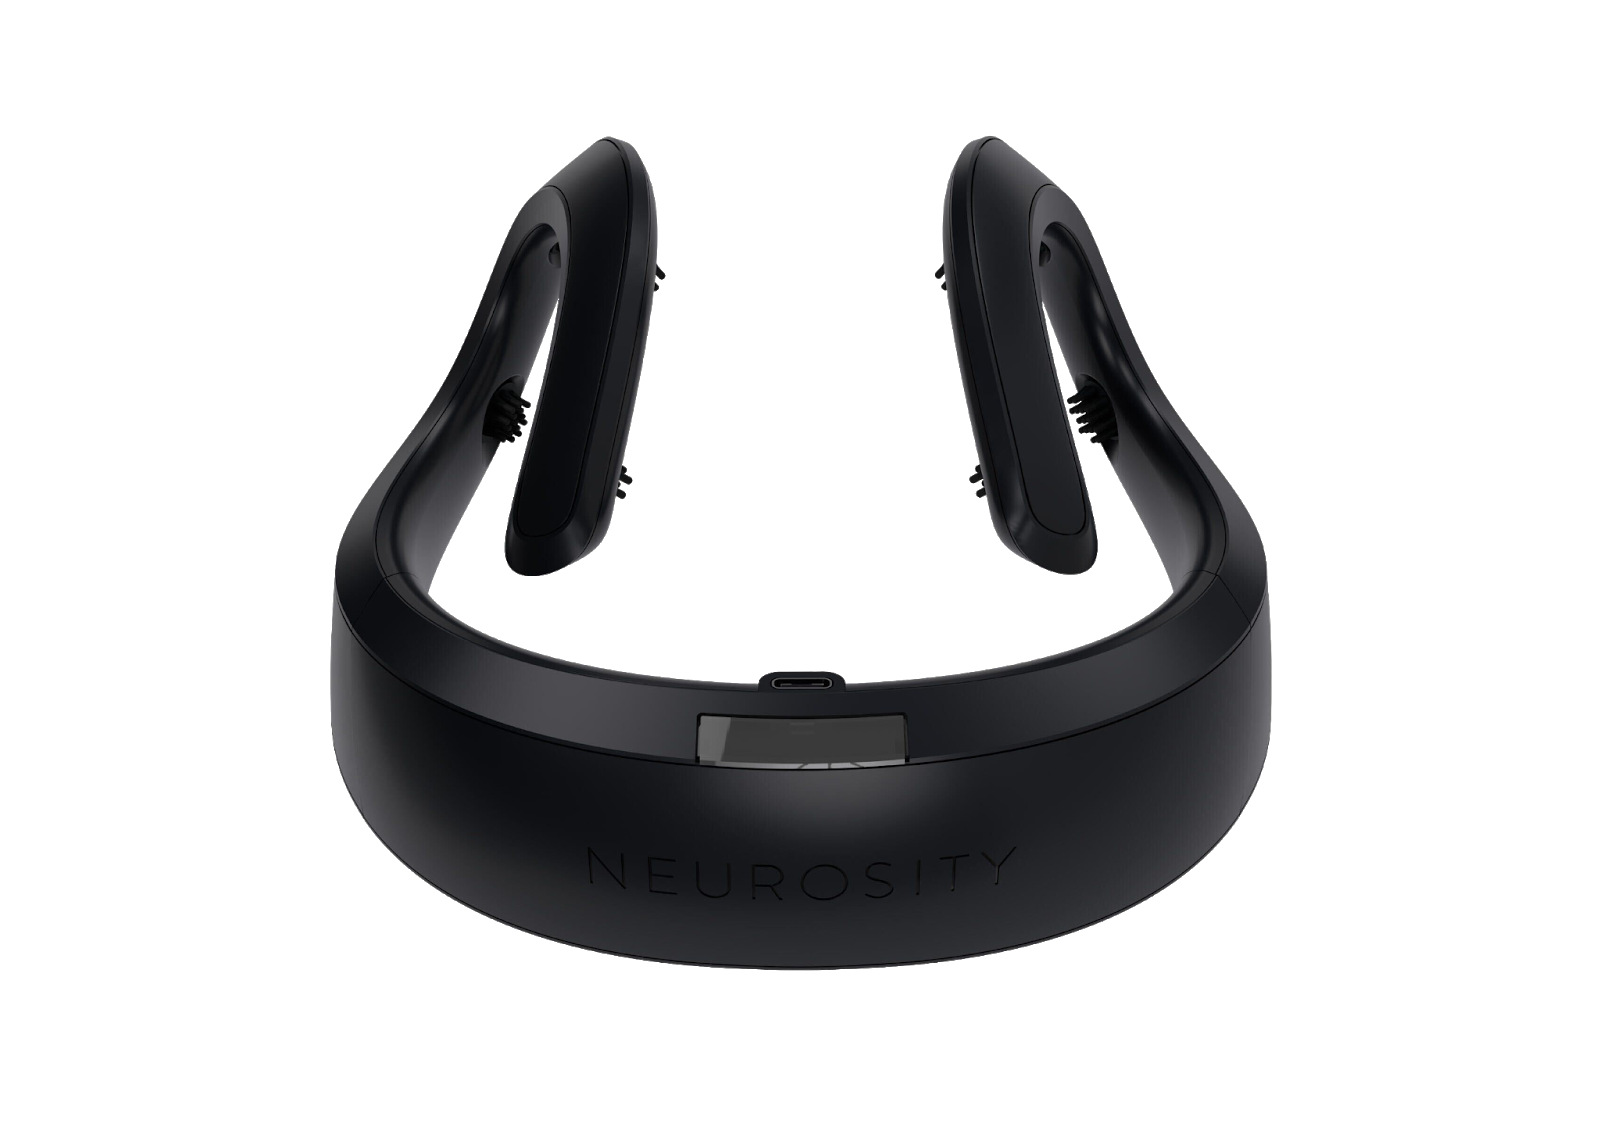
\includegraphics[trim=200 150 200 100,clip,width=3cm]{./img/crown-1.png}
            \\ Neurosity Crown
        \end{column}

        \begin{column}{0.33\textwidth}
            \centering
            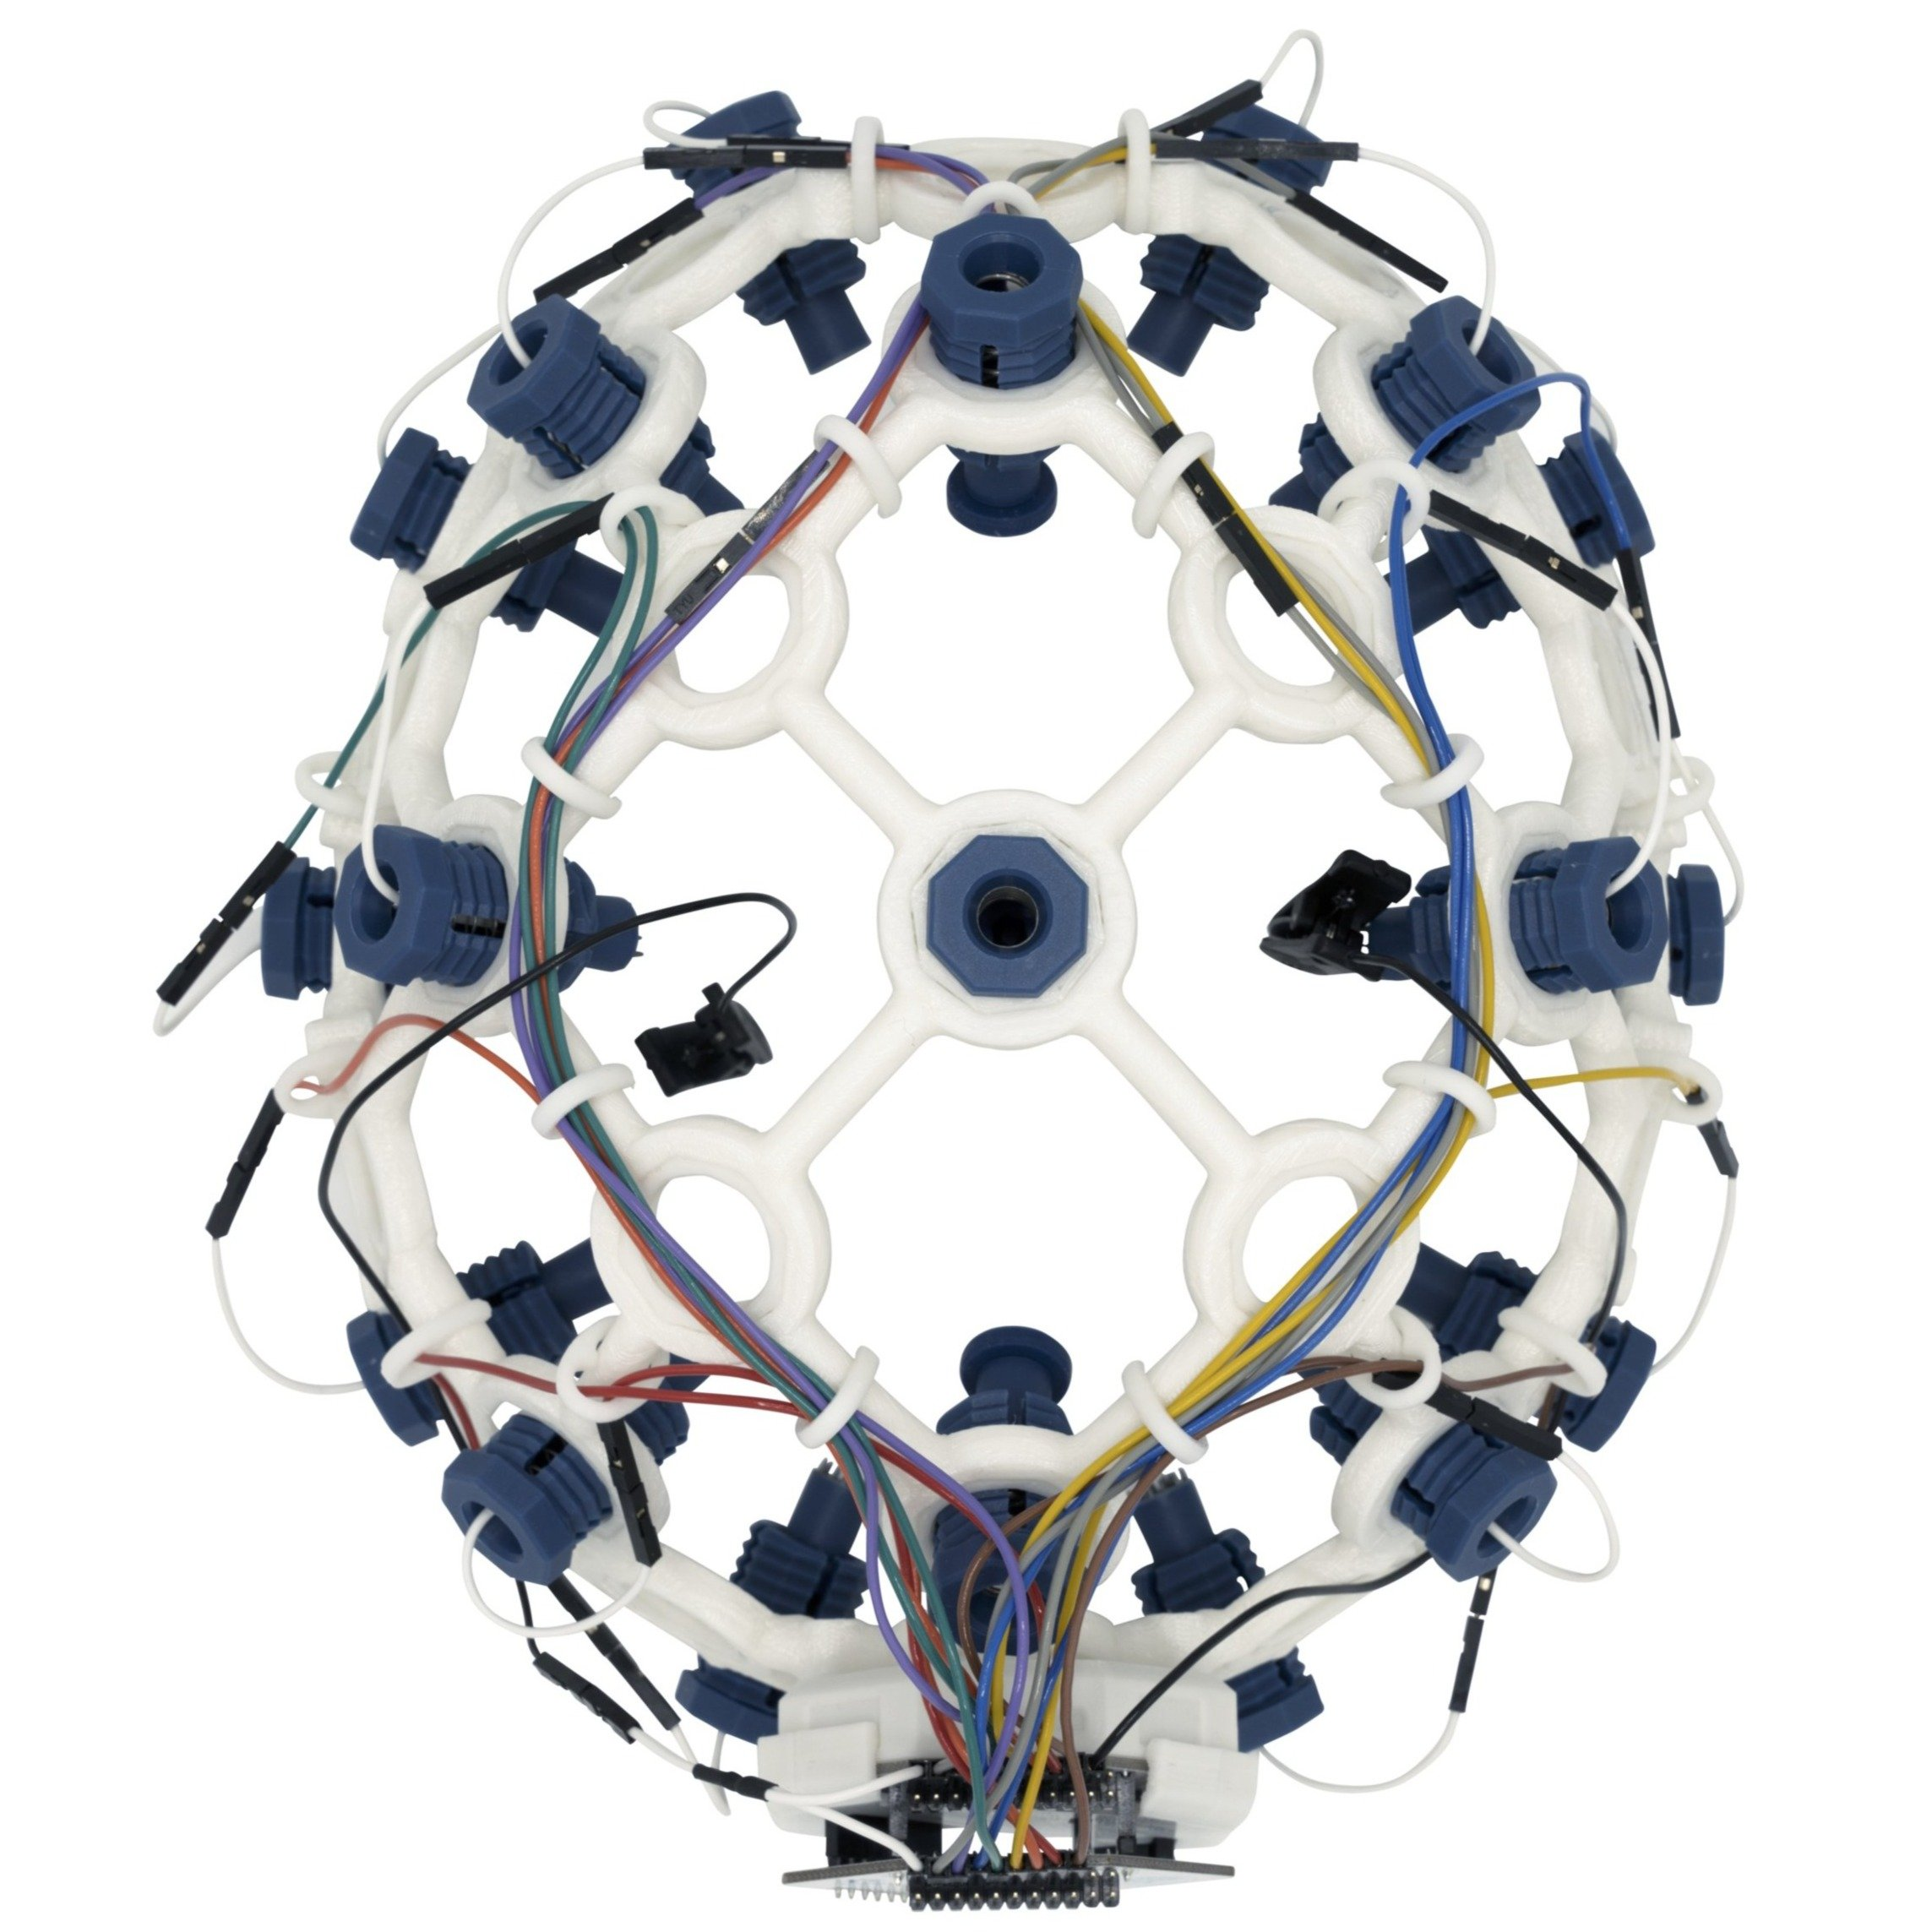
\includegraphics[width=3cm]{./img/openbci-cyton.jpg}
            \\ OpenBCI Cyton + Ultracortex
        \end{column}
    \end{columns}

    \vspace{-5mm}
    \begin{adjustbox}{width=\textwidth,center,float=table}
        \begin{table}[H]
    \centering
    \begin{tabular}{llcrr}
        \toprule
        Manufacturer
        & Device
        & Channels
        & Sampling rate
        & Comfort
        \\
        \midrule
        InteraXon
        & Muse S (2020)
        & 4
        & 256Hz
        & High
        \\
        Neurosity
        & Crown (2021)
        & 8
        & 256Hz
        & Medium
        \\
        OpenBCI
        & Cyton (2013) + Ultracortex
        & 8--16
        & 125--250Hz
        & Low
        \\
        \bottomrule
    \end{tabular}
    \caption{Devices used}\label{table:devices}
\end{table}

    \end{adjustbox}
\end{frame}

\subsection{Collection}
\begin{frame}{Method}
    \framesubtitle{Collection $>$ Code vs prose}
    {
        \small
        \begin{figure}[H]
    \centering
    \begin{tabular}{cc}
        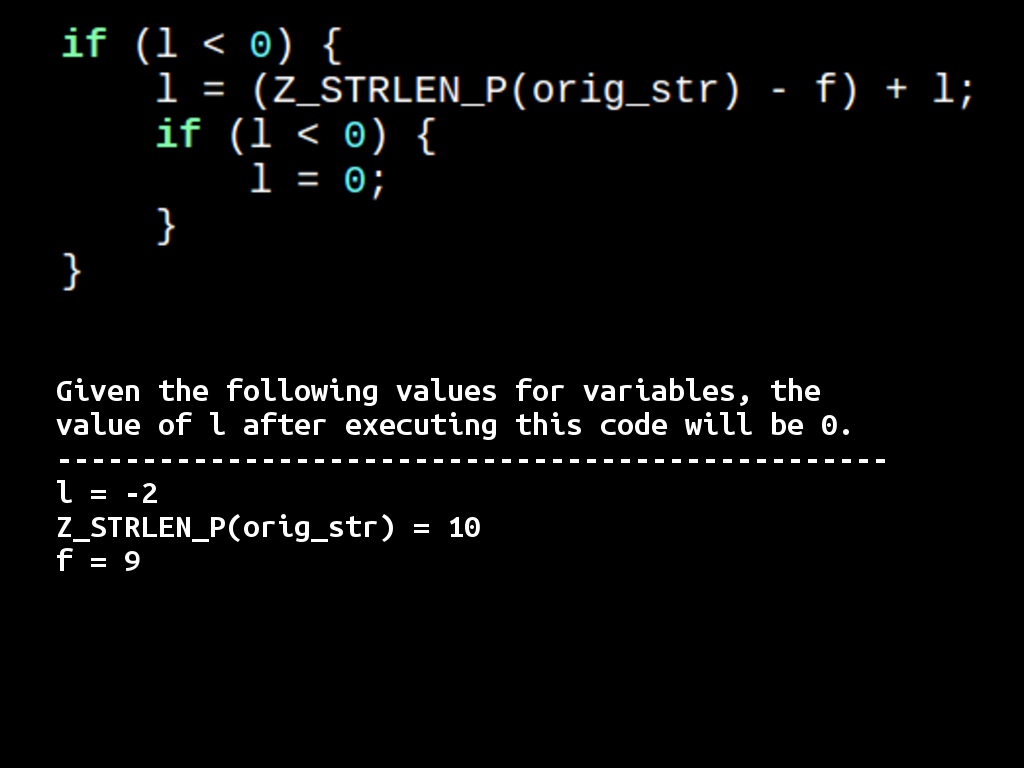
\includegraphics[trim=25 160 0 0,clip,width=0.45\linewidth]{img/final-1-1.png}
        &
        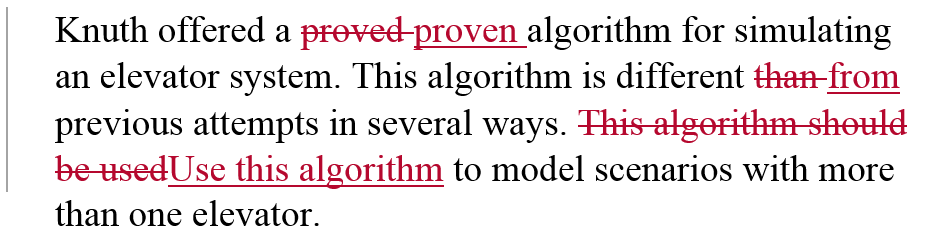
\includegraphics[trim=20 0 20 0,clip,width=0.45\linewidth]{img/bugs_1.PNG}
        \\
        (a) Code comprehension
        &
        (b) Prose review
    \end{tabular}
    \caption{Sample of the tasks used as stimuli.}\label{fig:tasks}
\end{figure}

    }
\end{frame}

\subsection{Analysis}
\begin{frame}{Method}
    \framesubtitle{Analysis $>$ Performance evaluation}
    \begin{itemize}
        \item Studies using EEG often use \emph{balanced accuracy} (BAC).
        \item Balanced accuracy deals with imbalanced datasets.
    \end{itemize}

    \vspace{2em}

    For binary classification, BAC is defined as:
    $$BAC = \frac{TP + TN}{2}$$
    This implies that, for the binary case, $BAC = 0.5$ is no better than chance.
\end{frame}

\begin{frame}{Method}
    \framesubtitle{Analysis $>$ Validation}
    To ensure our classifier generalizes across subjects, we perform \emph{Leave-One-Run-Out} (LORO) cross validation.
    \vspace{1em}
    \definecolor{train}{RGB}{163, 206, 255}
\definecolor{test}{RGB}{255, 181, 84}
\begin{table}[h]
    \centering
    \begin{tabular}{lcccc}
        \toprule
               & Subject 1 & Subject 2 & Subject 3 & Subject 4 \\
        \midrule
        Fold 1 & \cellcolor{test}     & \multicolumn{3}{c}{\cellcolor{train}} \\
        Fold 2 & \cellcolor{train} & \cellcolor{test}     & \multicolumn{2}{c}{\cellcolor{train}     } \\
        Fold 3 & \multicolumn{2}{c}{\cellcolor{train}     } & \cellcolor{test}     & \cellcolor{train} \\
        Fold 4 & \multicolumn{3}{c}{\cellcolor{train}} & \cellcolor{test}     \\
        \bottomrule
    \end{tabular}
    \caption{Example of Leave-One-Run-Out cross validation with 4 subjects. For each fold, subjects marked \textcolor{NavyBlue}{\textbf{blue}} are used for training and subjects marked \textcolor{BurntOrange}{\textbf{orange}} are used for testing.}\label{table:loro}
\end{table}

\end{frame}

\section{Results}
\begin{frame}{Results}
    Our results are:
    {
        \small
        \begin{table}[h]
    \centering
    \begin{tabular}{lcccc}
        \toprule
        & \multicolumn{2}{c}{\textbf{Riemannian}} & \multicolumn{2}{c}{\textbf{Bandpower}} \\
        \cmidrule(lr){2-3}
        \cmidrule(lr){4-5}
        \textbf{Subject} & Window-level & Epoch-level & Window-level & Epoch-level \\
        \midrule
        \#0 & 0.673 & 0.727 & 0.511 & 0.541 \\
        \#1 & 0.895 & 0.955 & 0.689 & 0.809 \\
        \#5 & 0.616 & 0.542 & 0.628 & 0.750 \\
        \#6 & 0.864 & 0.908 & 0.739 & 0.737 \\
        \#7 & 0.749 & 0.900 & 0.733 & 0.733 \\
        \midrule
        Median & 0.749 & 0.900 & 0.689 & 0.737 \\
        \bottomrule
    \end{tabular}
    \caption{The balanced accuracy for each LORO fold/subject. Excluding subjects 3, 4, 8, 9, and 10.}\label{table:bac-selective}
\end{table}

    }
\end{frame}

\begin{frame}{Results}
    \framesubtitle{Compared to previous studies}
    \
    {
        \small
        \begin{table}[h]
    \begin{center}
        \begin{tabular}{lcccc}
            \toprule
            & \multicolumn{2}{c}{\textbf{This study}} & \multirow{2}{*}{\textbf{Fucci et al.}} & \multirow{2}{*}{\textbf{Floyd et al.}} \\
            \cmidrule(lr){2-3}
            & Riemannian & Bandpower & & \\
            \midrule
            Overall & 0.75 & 0.69 & 0.66 & 0.79 \\
            \bottomrule
        \end{tabular}
        \caption{Result comparison between the previous studies and this study. Best balanced accuracy scores are reported. For this study, we used the best window-level score. For Fucci et al.\ we chose the best EEG-only score.}\label{table:compare-results}
    \end{center}
\end{table}

    }
\end{frame}

\placelogofalse{}
\begin{frame}{Results}
    \framesubtitle{Data overview}
    {
        \tiny
        \begin{figure}
    \centering
    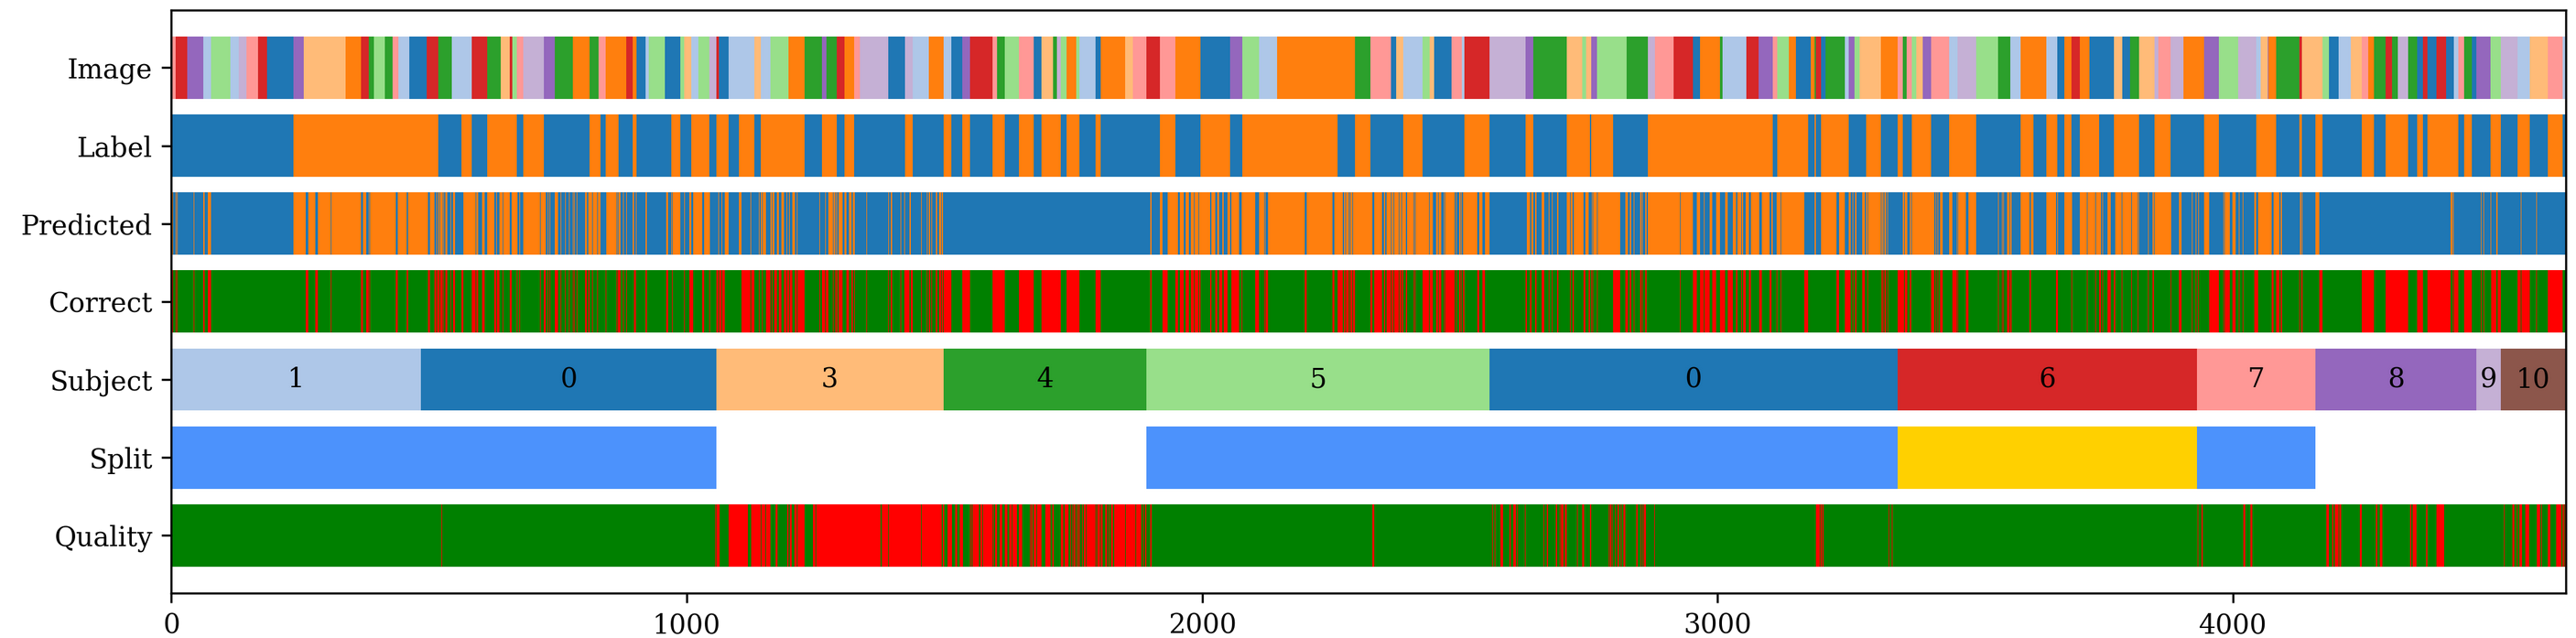
\includegraphics[width=\linewidth]{img/timebars.png}
    \caption{Visualization of the labeled data with classifications from one example subject-fold. Shows the \emph{Image} (stimuli), the class \emph{Label} for that stimuli (\textcolor{NavyBlue}{\textbf{blue}} is code, \textcolor{BurntOrange}{\textbf{orange}} is prose), the \emph{Predicted} class, whether the prediction is \emph{Correct}, the \emph{Subject}, the \emph{Split}/Fold (\textcolor{NavyBlue}{\textbf{blue}} shows the training set, \textcolor{Goldenrod}{\textbf{yellow}} the test set), and our threshold measure for signal \emph{Quality} (\textcolor{Green}{\textbf{green}} indicates acceptable quality). The x-axis is the window index, sorted by acquisition time.
    \\
    \vspace{0.5em}
    It can be seen that (1) subjects \#3 and \#4 have bad signal quality, and have therefore been excluded from the training set. (2) The subjects \#9 and \#10 have also been excluded from training due to issues during data collection. (3) For subject \#1 the stimuli images were not shuffled. (4) Subject \#0 appears twice, as they did two sessions (using unseen stimuli).}\label{fig:timebars}
\end{figure}

    }
\end{frame}
\placelogotrue{}

\section{Discussion}
\begin{frame}{Discussion}
\end{frame}

\subsection*{Applications}
\begin{frame}{Discussion}
    \framesubtitle{Applications}
\end{frame}

\subsection*{Threats to validity}
\begin{frame}{Discussion}
    \framesubtitle{Threats to validity}
\end{frame}

\subsection*{Ethical considerations}
\begin{frame}{Discussion}
    \framesubtitle{Ethical considerations}
\end{frame}

\section{Conclusions}
\begin{frame}{Conclusions}
    We conclude that bla bla bla

    \begin{itemize}
        \item TODO
    \end{itemize}
\end{frame}

\subsection{Future work}
\begin{frame}{Conclusions}
    \framesubtitle{Future work}
\end{frame}

\section*{References}
\begin{frame}[allowframebreaks]{References}
    \AtNextBibliography{\scriptsize}
    \printbibliography[category=cited]
\end{frame}

\end{document}
